\documentclass[11pt,a4paper]{article}
\usepackage[margin=2.5cm]{geometry}
\usepackage[T1]{fontenc}
\usepackage{lmodern}
\usepackage{amsmath,amssymb}
\usepackage{booktabs,tabularx,array}
\usepackage{graphicx}
\usepackage{xcolor}
\usepackage[round]{natbib}
\usepackage{tikz}
\usetikzlibrary{arrows.meta,positioning,calc}
\usepackage{caption}
\usepackage[colorlinks=true,allcolors=blue!50!black]{hyperref}
\graphicspath{{../stats/figs/}}
\captionsetup{font=small,labelfont=bf}

% ---- figures / tables produced by the scripts; the article compiles even before they exist
\newcommand{\maybefig}[3]{% file, width, caption-label
  \IfFileExists{../stats/figs/#1}{\includegraphics[width=#2\textwidth]{#1}}%
  {\fbox{\parbox{0.8\textwidth}{\centering\small [figure \texttt{\detokenize{#1}} not generated yet -- run \texttt{analyze.py}]}}}}
\newcommand{\maybetab}[1]{%
  \IfFileExists{../stats/tabs/#1}{\input{../stats/tabs/#1}}%
  {\fbox{\parbox{0.8\textwidth}{\centering\small [table \texttt{\detokenize{#1}} not generated yet -- run \texttt{analyze.py}]}}}}

\newcommand{\E}{\mathbb{E}}
\newcommand{\R}{\mathbb{R}}
\newcommand{\dd}{\,\mathrm{d}}
\newcommand{\Tb}{\bar T}

\title{\textbf{A Fractional Delayed Impulsive Model of Interacting Earthquake Faults:\\ Probabilistic Forecasting, Inference and Statistical Validation}}
\author{Mohamad Yamen Al-Mohamad\\
\small Department of Statistics, University of Tabriz, Tabriz, Iran\\
\small \texttt{yamenmohamad@tabrizu.ac.ir}}
\date{\today}

%%% ---------- Figure A: the problem ----------
\newcommand{\figProblem}{%
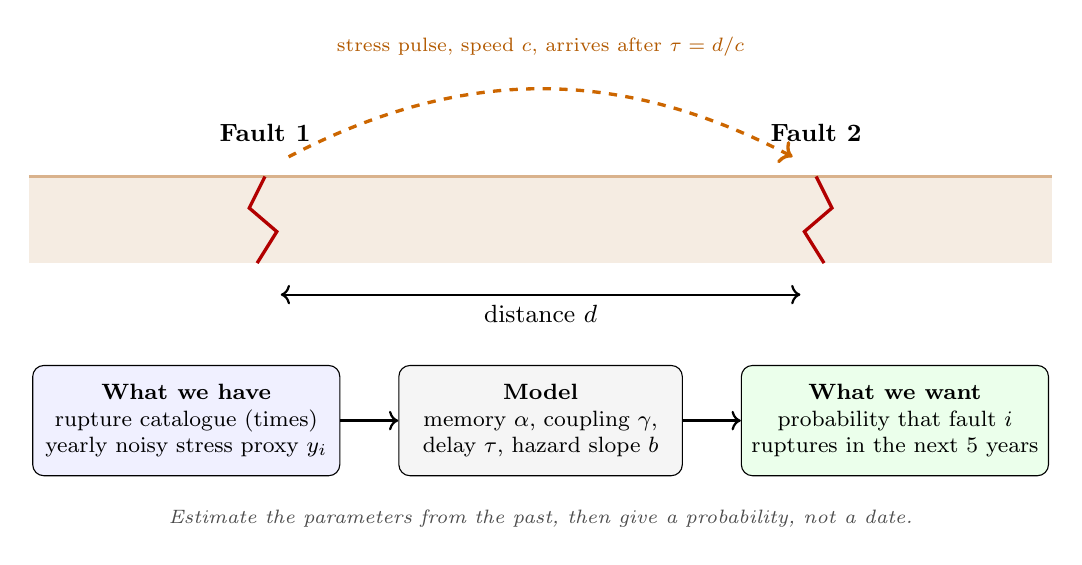
\begin{tikzpicture}[x=1cm,y=1cm,
  lab/.style={font=\small,align=center},
  bx/.style={font=\footnotesize,align=center,draw,rounded corners,minimum height=1.4cm},
  note/.style={font=\scriptsize,align=center,text=black!70}]
  % ground
  \fill[brown!15] (0,0) rectangle (13,-1.1);
  \draw[brown!60,thick] (0,0)--(13,0);
  % fault 1 and 2 (zig-zag lines going down)
  \draw[red!70!black,very thick] (3,0)--(2.8,-0.4)--(3.15,-0.7)--(2.9,-1.1);
  \draw[red!70!black,very thick] (10,0)--(10.2,-0.4)--(9.85,-0.7)--(10.1,-1.1);
  \node[lab] at (3,0.55) {\textbf{Fault 1}};
  \node[lab] at (10,0.55) {\textbf{Fault 2}};
  % distance
  \draw[<->,thick] (3.2,-1.5)--node[below,lab]{distance $d$}(9.8,-1.5);
  % pulse
  \draw[->,orange!80!black,very thick,dashed] (3.3,0.25) .. controls (5.5,1.4) and (7.5,1.4) .. (9.7,0.25);
  \node[note,orange!70!black] at (6.5,1.65) {stress pulse, speed $c$, arrives after $\tau=d/c$};
  % what we see
  \node[bx,fill=blue!6,minimum width=3.9cm] (obs) at (2.0,-3.1)
     {\textbf{What we have}\\ rupture catalogue (times)\\ yearly noisy stress proxy $y_i$};
  \node[bx,fill=gray!8,minimum width=3.6cm] (mod) at (6.5,-3.1)
     {\textbf{Model}\\ memory $\alpha$, coupling $\gamma$,\\ delay $\tau$, hazard slope $b$};
  \node[bx,fill=green!8,minimum width=3.9cm] (q) at (11.0,-3.1)
     {\textbf{What we want}\\ probability that fault $i$\\ ruptures in the next 5 years};
  \draw[->,thick] (obs)--(mod);
  \draw[->,thick] (mod)--(q);
  \node[note] at (6.5,-4.35) {\emph{Estimate the parameters from the past, then give a probability, not a date.}};
\end{tikzpicture}}

%%% ---------- Figure B: stress cycle, memory, hazard ----------
\newcommand{\figCycle}{%
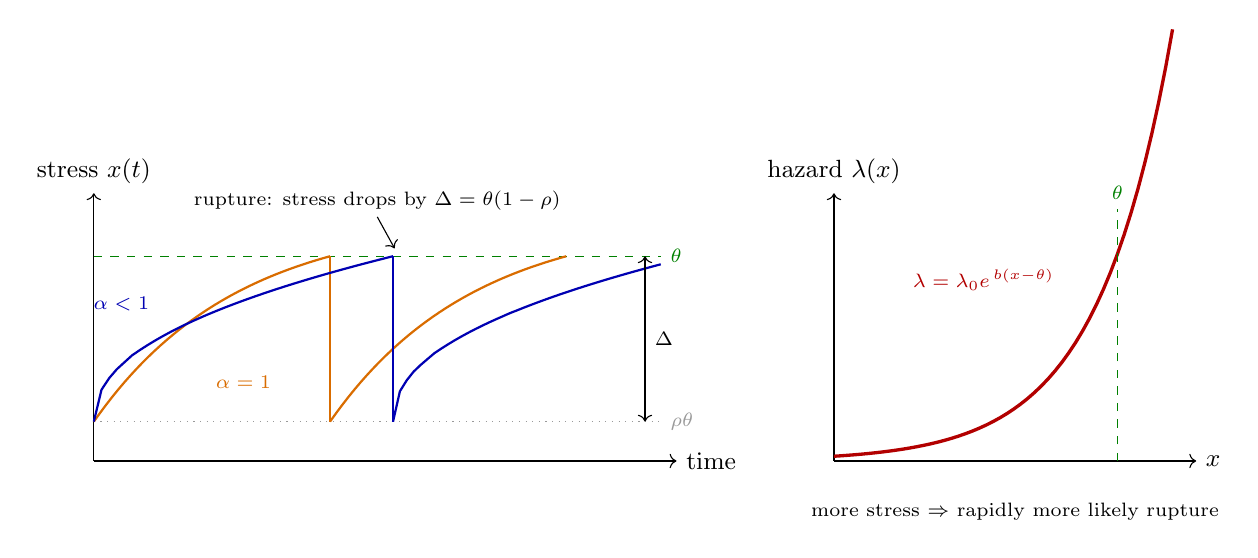
\begin{tikzpicture}[x=1.0cm,y=1.0cm,font=\small]
  % --- left: stress cycles
  \draw[->] (0,0)--(7.4,0) node[right]{time};
  \draw[->] (0,0)--(0,3.4) node[above]{stress $x(t)$};
  \draw[green!50!black,dashed] (0,2.6)--(7.2,2.6) node[right,font=\scriptsize]{$\theta$};
  \draw[black!40,dotted] (0,0.5)--(7.2,0.5) node[right,font=\scriptsize]{$\rho\theta$};
  % no memory (alpha=1): classical saturating curve, two cycles
  \draw[thick,orange!85!black] plot[domain=0:3,samples=40] (\x,{0.5+2.1*(1-exp(-0.55*\x))/(1-exp(-0.55*3))});
  \draw[thick,orange!85!black] (3,2.6)--(3,0.5);
  \draw[thick,orange!85!black] plot[domain=0:3,samples=40] ({3+\x},{0.5+2.1*(1-exp(-0.55*\x))/(1-exp(-0.55*3))});
  % with memory: fast start, slow end (power law)
  \draw[thick,blue!70!black] plot[domain=0:3.8,samples=40] (\x,{0.5+2.1*(\x/3.8)^0.45});
  \draw[thick,blue!70!black] (3.8,2.6)--(3.8,0.5);
  \draw[thick,blue!70!black] plot[domain=0:3.4,samples=40] ({3.8+\x},{0.5+2.1*(\x/3.8)^0.45});
  % drop
  \draw[<->] (7.0,0.5)--node[right,font=\scriptsize]{$\Delta$}(7.0,2.6);
  \node[font=\scriptsize,orange!85!black] at (1.9,1.0) {$\alpha=1$};
  \node[font=\scriptsize,blue!70!black] at (0.35,2.0) {$\alpha<1$};
  \node[font=\scriptsize,align=center] at (3.6,3.3) {rupture: stress drops by $\Delta=\theta(1-\rho)$};
  \draw[->,font=\scriptsize] (3.6,3.1)--(3.82,2.7);
  % --- right: hazard
  \begin{scope}[xshift=9.4cm]
    \draw[->] (0,0)--(4.6,0) node[right]{$x$};
    \draw[->] (0,0)--(0,3.4) node[above]{hazard $\lambda(x)$};
    \draw[very thick,red!70!black] plot[domain=0:4.3,samples=50] (\x,{0.06*exp(1.05*\x)});
    \draw[green!50!black,dashed] (3.6,0)--(3.6,3.2) node[above,font=\scriptsize]{$\theta$};
    \node[font=\scriptsize,red!70!black,align=center] at (1.9,2.3) {$\lambda=\lambda_0e^{\,b(x-\theta)}$};
    \node[font=\scriptsize,align=center] at (2.3,-0.65) {more stress $\Rightarrow$ rapidly more likely rupture};
  \end{scope}
\end{tikzpicture}}

%%% ---------- Figure C: delayed pulse timeline ----------
\newcommand{\figDelay}{%
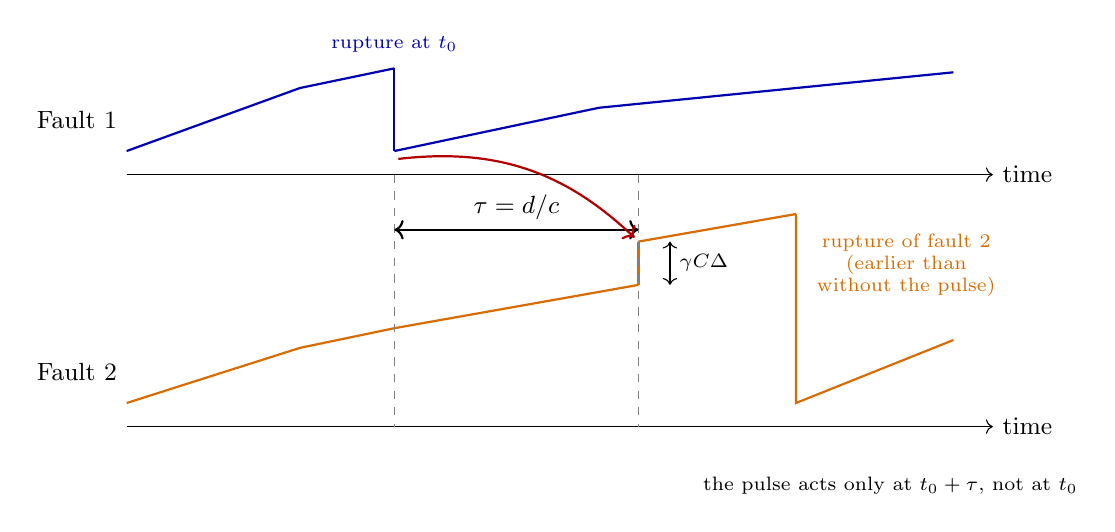
\begin{tikzpicture}[x=1cm,y=1cm,font=\small]
  % fault 1 axis
  \draw[->] (0,3.6)--(11,3.6) node[right]{time};
  \node[left] at (0,4.3) {Fault 1};
  \draw[blue!70!black,thick] (0,3.9)--(2.2,4.7)--(3.4,4.95);
  \draw[blue!70!black,thick] (3.4,4.95)--(3.4,3.9);
  \draw[blue!70!black,thick] (3.4,3.9)--(6,4.45)--(10.5,4.9);
  \node[blue!70!black,font=\scriptsize] at (3.4,5.25) {rupture at $t_0$};
  % fault 2 axis
  \draw[->] (0,0.4)--(11,0.4) node[right]{time};
  \node[left] at (0,1.1) {Fault 2};
  \draw[orange!85!black,thick] (0,0.7)--(2.2,1.4)--(3.4,1.65)--(6.5,2.2);
  \draw[orange!85!black,thick] (6.5,2.2)--(6.5,2.75);       % jump gamma*C*Delta
  \draw[orange!85!black,thick] (6.5,2.75)--(8.5,3.1);
  \draw[orange!85!black,thick] (8.5,3.1)--(8.5,0.7)--(10.5,1.5);
  \node[orange!85!black,font=\scriptsize,align=center] at (9.9,2.45) {rupture of fault 2\\ (earlier than\\ without the pulse)};
  % delay arrows
  \draw[dashed,gray] (3.4,3.6)--(3.4,0.4);
  \draw[dashed,gray] (6.5,3.6)--(6.5,0.4);
  \draw[<->,thick] (3.4,2.9)--node[above]{$\tau=d/c$}(6.5,2.9);
  \draw[->,red!70!black,thick] (3.45,3.8) to[bend left=25] (6.45,2.8);
  \node[red!70!black,font=\scriptsize] at (4.4,3.4) {};
  \draw[<->] (6.9,2.2)--node[right,font=\scriptsize]{$\gamma C\Delta$}(6.9,2.75);
  \node[font=\scriptsize,align=center] at (9.7,-0.35) {the pulse acts only at $t_0+\tau$, not at $t_0$};
\end{tikzpicture}}

%%% ---------- Figure D: inference pipeline ----------
\newcommand{\figPipeline}{%
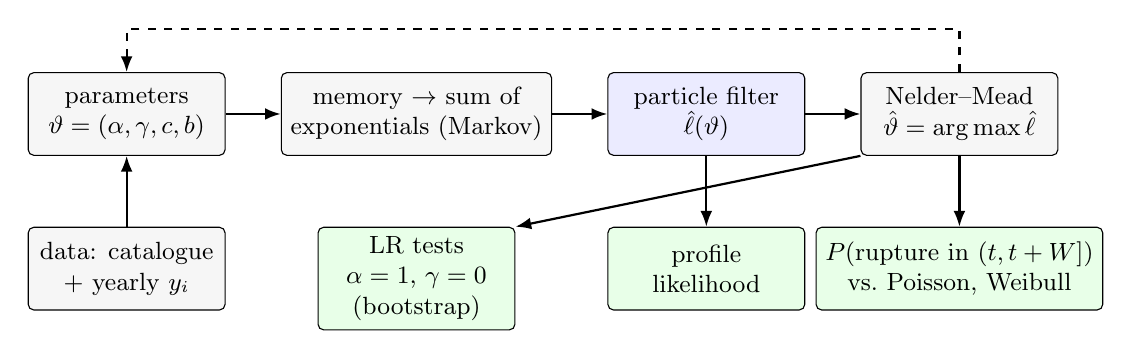
\begin{tikzpicture}[node distance=0.55cm and 0.7cm,
  box/.style={draw,rounded corners=2pt,align=center,minimum height=1.05cm,minimum width=2.5cm,font=\small,fill=gray!7},
  hi/.style={box,fill=blue!8},
  outb/.style={box,fill=green!9},
  arr/.style={-{Latex[length=2mm]},thick}]
  \node[box] (par) {parameters\\ $\vartheta=(\alpha,\gamma,c,b)$};
  \node[box,right=of par] (soe) {memory $\to$ sum of\\ exponentials (Markov)};
  \node[hi,right=of soe] (pf) {particle filter\\ $\hat\ell(\vartheta)$};
  \node[box,right=of pf] (opt) {Nelder--Mead\\ $\hat\vartheta=\arg\max\hat\ell$};
  \node[box,below=0.9cm of par] (dat) {data: catalogue\\ + yearly $y_i$};
  \node[outb,below=0.9cm of soe] (lr) {LR tests\\ $\alpha=1$, $\gamma=0$\\ (bootstrap)};
  \node[outb,below=0.9cm of pf] (prof) {profile\\ likelihood};
  \node[outb,below=0.9cm of opt] (fc) {$P(\text{rupture in }(t,t+W])$\\ vs.\ Poisson, Weibull};
  \draw[arr] (par)--(soe); \draw[arr] (soe)--(pf); \draw[arr] (pf)--(opt);
  \draw[arr] (dat)--(par); 
  \draw[arr] (opt)--(fc); \draw[arr] (pf)--(prof); \draw[arr] (opt.south west)--(lr.north east);
  \draw[arr,dashed] (opt.north) -- ++(0,0.55) -| (par.north);
\end{tikzpicture}}

\begin{document}
\maketitle

\begin{abstract}
We propose a stochastic dynamical model for a system of interacting earthquake faults in which the tectonic stress on each fault has \emph{long memory} (a Caputo fractional derivative of order $\alpha\in(0,1]$), ruptures are \emph{impulses} that reset the stress of the failing fault, and each rupture sends a \emph{delayed} stress pulse to the neighbouring fault after a travel time $\tau=d/c$. Earthquakes occur at a stress-dependent hazard, so the model yields probabilities of rupture in a future window rather than a single deterministic prediction. Parameters are estimated by maximum likelihood, the likelihood being approximated by a bootstrap particle filter on a sum-of-exponentials representation of the fractional kernel. We describe a complete statistical protocol: a replication study of the estimator (bias, SD, RMSE), a likelihood-ratio test of memory ($H_0:\alpha=1$) calibrated by parametric bootstrap because $\alpha=1$ lies on the boundary of the parameter space, a test of interaction ($H_0:\gamma=0$), profile likelihoods, robustness to a misspecified reference recurrence time, and an out-of-sample evaluation of the window forecasts (Brier score, log score, AUC, reliability) against Poisson, Weibull-renewal and no-memory benchmarks. The scope and limitations of the study---in particular that stress is observed directly in the simulations---are stated explicitly.
\end{abstract}

\noindent\textbf{Keywords:} fractional differential equations, impulsive systems, time delay, earthquake forecasting, particle filter, likelihood-ratio test on the boundary.

%==============================================================
\section{Introduction}
Earthquake recurrence is classically described by renewal models (a fault ruptures, stress is reset, and the next event is drawn from a recurrence distribution) or by point-process models such as the Hawkes/ETAS family \citep{Hawkes1971,Ogata1988}. Two physical features are awkward in these frameworks: (i) the loading of a fault is not memoryless---the crust is viscoelastic, so the present stress depends on the whole loading history; and (ii) faults interact through stress transfer that travels at finite speed, so the effect of one rupture on its neighbour is \emph{delayed}. Spring--block descriptions go back to \citet{BurridgeKnopoff1967}, and the elastic-rebound idea to \citet{Reid1910}.

Fractional calculus gives a compact way to encode memory \citep{Podlubny1999,Diethelm2010}: the Caputo derivative of order $\alpha<1$ weights the past with the power-law kernel $t^{\alpha-1}/\Gamma(\alpha)$. This paper combines three ingredients in one model---fractional memory, impulsive ruptures, and delayed coupling---and, more importantly, asks the statistical questions that a model of this kind must answer before it is taken seriously: \emph{can its parameters be recovered from data, can memory and interaction be detected, and do the forecasts beat simple benchmarks out of sample?}

\begin{figure}[t]
\centering\resizebox{\textwidth}{!}{\figProblem}
\caption{The problem. Two faults a distance $d$ apart exchange stress; we observe the past ruptures and a noisy stress proxy and want a probability of rupture in a future window, not a single date.}\label{fig:problem}
\end{figure}

\begin{figure}[t]
\centering\maybefig{fault_map.pdf}{0.85}{}
\caption{A real example of the setting: two neighbouring active faults (blue and orange) with the closest-approach distance $d$ used in $\tau=d/c$. Fault traces from the GEM Global Active Faults Database \citep{StyronPagani2020}; map drawn with \texttt{cartopy}. The two traces are automatically chosen as distinct fault traces (about $100$ km long each) whose closest approach is about $30$\,km, the value of $d$ used in the simulations; the simulation study itself uses synthetic data, and the map only illustrates the geometry. Neighbouring in space does not by itself establish mechanical interaction.}\label{fig:map}
\end{figure}

\paragraph{Contributions.}
(1) A two-fault model with fractional memory, impulses and pulse delay, together with a calibration of the loading rate from a reference recurrence time. (2) A likelihood by particle filtering with an accurate sum-of-exponentials kernel. (3) A reproducible statistical protocol, with hypothesis tests that respect the boundary problem at $\alpha=1$. (4) An honest statement of what the simulation evidence does and does not establish.

%==============================================================
\section{Related work and comparison}\label{sec:related}
We organise related work by the modelling feature it shares with the present model, and then summarise the comparison in Table~\ref{tab:related}.

\paragraph{Renewal and stress-release models.}
Classical recurrence models treat the inter-event time of a fault as an i.i.d.\ draw from a Weibull, lognormal or Brownian-passage-time law \citep{Matthews2002}; they have no mechanism for interaction and use elapsed time only. The \emph{stress release model} of \citet{VereJones1978} (see also \citealp{ZhengVereJones1991}) is closer in spirit: stress increases linearly, earthquakes occur at a stress-dependent hazard $\lambda=\exp(a+b\,x)$ and release stress. The \emph{linked} stress-release model couples several regions through stress transfer \citep{LuVereJones2000,Bebbington2003} and has a well-developed likelihood theory. Our hazard \eqref{eq:hazard} has the same exponential-in-stress form, so the present model can be seen as a stress-release model in which (i) loading is not linear but has fractional memory and saturation, and (ii) coupling is split into an instantaneous part and a \emph{delayed} pulse. In the linked model coupling is instantaneous and memoryless, and stress is a deterministic function of the catalogue (no latent state, no particle filter).

\paragraph{Self-exciting point processes.}
The Hawkes process and ETAS \citep{Hawkes1971,Ogata1988} are the standard operational forecasting tools. They model clustering (aftershocks) through a power-law triggering kernel; memory enters as event-to-event triggering, not as accumulated tectonic stress, and they say little about the quasi-periodic behaviour of large characteristic earthquakes. Our model targets the opposite regime (large, recurrent events on a few faults), and ETAS-type clustering is not included; the two are complementary.

\paragraph{Physics-based stress transfer.}
Coulomb stress transfer \citep{Stein1999} and rate-and-state seismicity models \citep{Dieterich1994} compute how a rupture changes stress, and hence the earthquake rate, on neighbouring faults, including time-dependent effects of friction. They require fault geometry, slip distributions and constitutive parameters that are rarely available; our model replaces this by two effective parameters ($\gamma$, $c$) that can be estimated, at the price of physical detail. Spring--block models \citep{BurridgeKnopoff1967} and quasi-dynamic simulators produce interacting-fault sequences, but are not formulated for statistical inference from catalogues.

\paragraph{Fractional and delayed earthquake models.}
Fractional calculus has been used for viscoelastic wave propagation, e.g.\ attenuation and dispersion under Atangana--Baleanu dynamics \citep{DemirKocyigit2025}, but that work concerns wave propagation without rupture, faults or catalogues. A paper on \emph{delayed and fractional-order dynamics of a model for earthquake induced by stress perturbations} \citep{PhysScr2024} studies the dynamics of a low-dimensional model with delay and fractional order (we could not access the full text, so our statement of its content is limited to its title and abstract-level description and should be verified). The closest recent work we found is the preprint of \citet{Chishtie2026}, a hierarchical fractional $N$-body framework for Coulomb stress evolution in fault networks. It uses a fractional evolution equation whose order is tied to the number of interacting bodies, $\alpha_k=2-2/(N_k+1)$, and derives scaling laws (Omori--Utsu exponent, spatial stress decay, Gutenberg--Richter $b$-value) \emph{without free parameters}; it builds on the time-dependent stress-recovery model of \citet{DahmHainzl2022}. According to its posted text it contains no delay, no probabilistic forecasting, no likelihood-based inference, and its observational test is still to be done (only qualitative comparisons with two events). Our approach is different in kind: $\alpha$ is a \emph{parameter estimated from data} (and tested against $\alpha=1$), delays are explicit, ruptures are impulses, and the output is a forecast probability evaluated out of sample. The two are therefore complementary: a theory that predicts $\alpha$ from network structure could provide a prior or a constraint for the estimation developed here.

\begin{table}[t]
\centering\scriptsize
\setlength{\tabcolsep}{2pt}
\begin{tabularx}{\textwidth}{>{\raggedright\arraybackslash}p{3.2cm}*{6}{>{\centering\arraybackslash}X}}
\toprule
Approach & Memory & Interaction & Delay & Latent stress & Likelihood inference & Prob.\ forecast\\
\midrule
Renewal (Weibull/BPT) & -- & -- & -- & -- & yes & yes\\
Stress-release \citep{VereJones1978} & -- & -- & -- & deterministic & yes & yes\\
Linked stress-release \citep{LuVereJones2000,Bebbington2003} & -- & instantaneous & -- & deterministic & yes & yes\\
ETAS/Hawkes \citep{Ogata1988} & power-law triggering & yes & -- & -- & yes & yes\\
Coulomb/rate-state \citep{Stein1999,Dieterich1994} & friction only & physical & -- & physical & rarely & via rates\\
Fractional $N$-body \citep{Chishtie2026} & fractional & yes & -- & deterministic & -- & --\\
\textbf{This paper} & fractional, estimated $\alpha$ & continuous + delayed pulse & yes, $\tau=d/c$ & stochastic, filtered & yes (particle filter) & yes\\
\bottomrule
\end{tabularx}
\caption{Comparison with related approaches. Entries for other work reflect the cited sources as we understood them and should be checked against the full texts before submission.}\label{tab:related}
\end{table}

\paragraph{What is and is not claimed.}
We do not claim that the present model forecasts better than ETAS or physics-based models on real catalogues; this has not been tested. The claims are structural (a single model with memory, delay and impulses with a tractable likelihood) and statistical (parameter recovery, tests and benchmark comparison \emph{in simulation}, Section~\ref{sec:results}). Head-to-head comparison with the stress-release model on real data is the most informative next experiment; since the stress-release model is a special case without memory or delay, it is also a natural additional benchmark in the simulation protocol.

%==============================================================
\section{The model}
\subsection{Latent stress with fractional memory}
Let $x_i(t)$ be the (scalar, non-negative, dimensionless) tectonic stress on fault $i\in\{1,2\}$. Between ruptures it follows the Caputo-type Volterra equation
\begin{equation}\label{eq:volterra}
x_i(t)=x_i(0)+\frac{1}{\Gamma(\alpha)}\int_0^t (t-s)^{\alpha-1}F_i(x(s))\dd s+J_i(t),
\end{equation}
with drift/noise term
\begin{equation}\label{eq:F}
F_i = v_i-\beta x_i+\gamma\,(x_j-x_i)+\sigma_x\,\xi_i ,\qquad j\neq i,
\end{equation}
where $v_i$ is the tectonic loading rate, $\beta>0$ a relaxation rate, $\gamma\ge0$ the continuous coupling strength, $\xi_i$ white noise of intensity $\sigma_x$, and $\alpha\in(0,1]$ the memory order shared by both faults ($\alpha=1$ is the ordinary, memoryless ODE). The jump term $J_i(t)$ collects the impulses and is deliberately kept \emph{outside} the memory integral: a rupture is an instantaneous event, not a slowly decaying forcing. Initial stress is $x_i(0)=\rho\theta$ with $\theta$ the nominal failure threshold and $\rho\in(0,1)$ the residual fraction.

\subsection{Hazard, rupture and delayed pulses}
Fault $i$ ruptures at the hazard
\begin{equation}\label{eq:hazard}
\lambda_i(t)=\lambda_0\exp\!\big(b\,(x_i(t)-\theta)\big),\qquad \lambda_0=1,\ b>0,
\end{equation}
so that rupture becomes rapidly more likely as stress approaches and exceeds $\theta$. At a rupture of fault $i$ the stress drops by
\begin{equation}\label{eq:drop}
\Delta=\theta(1-\rho)\quad\Rightarrow\quad x_i\mapsto x_i-\Delta,
\end{equation}
and fault $j$ receives, after the travel time $\tau=d/c$ ($d$ = fault distance, $c$ = propagation speed), a stress pulse of size $\gamma C\Delta$ ($C$ a fixed transfer constant). The delay acts \emph{only on the pulse}; the smooth coupling term in \eqref{eq:F} is instantaneous. Figure~\ref{fig:schematic} summarises the structure.

\begin{figure}[t]
\centering
\resizebox{\textwidth}{!}{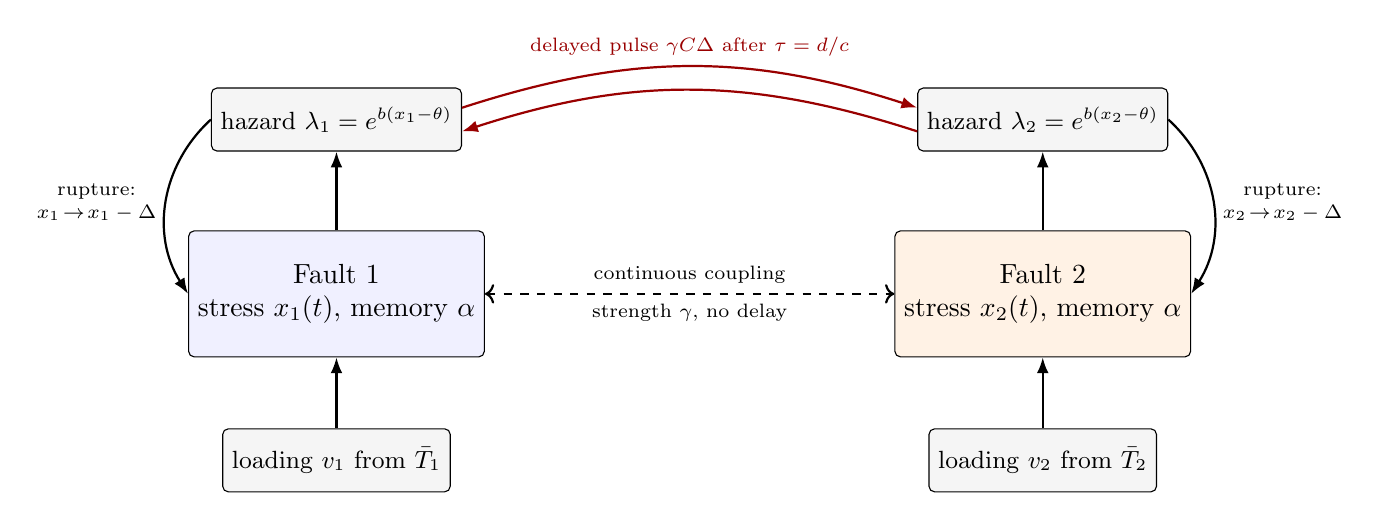
\begin{tikzpicture}[
  node distance=1.2cm,
  fault/.style={draw, rounded corners=2pt, minimum width=3.0cm, minimum height=1.6cm, align=center, fill=blue!6},
  fault2/.style={draw, rounded corners=2pt, minimum width=3.0cm, minimum height=1.6cm, align=center, fill=orange!10},
  proc/.style={draw, rounded corners=2pt, minimum width=2.6cm, minimum height=0.8cm, align=center, font=\small, fill=gray!8},
  arr/.style={-{Latex[length=2mm]}, thick},
  lab/.style={font=\scriptsize, align=center}
]
\node[fault] (F1) {Fault 1\\ stress $x_1(t)$, memory $\alpha$};
\node[fault2, right=5.2cm of F1] (F2) {Fault 2\\ stress $x_2(t)$, memory $\alpha$};
% continuous coupling
\draw[arr, <->, dashed] (F1.east) -- node[above, lab] {continuous coupling} node[below, lab] {strength $\gamma$, no delay} (F2.west);
% loading
\node[proc, below=0.9cm of F1] (L1) {loading $v_1$ from $\bar T_1$};
\node[proc, below=0.9cm of F2] (L2) {loading $v_2$ from $\bar T_2$};
\draw[arr] (L1) -- (F1);
\draw[arr] (L2) -- (F2);
% hazard and rupture
\node[proc, above=1.0cm of F1] (H1) {hazard $\lambda_1=e^{b(x_1-\theta)}$};
\node[proc, above=1.0cm of F2] (H2) {hazard $\lambda_2=e^{b(x_2-\theta)}$};
\draw[arr] (F1) -- (H1);
\draw[arr] (F2) -- (H2);
\draw[arr, bend right=40] (H1.west) to node[left, lab] {rupture:\\ $x_1\!\to\!x_1-\Delta$} (F1.west);
\draw[arr, bend left=40] (H2.east) to node[right, lab] {rupture:\\ $x_2\!\to\!x_2-\Delta$} (F2.east);
% delayed pulses
\draw[arr, red!60!black, bend left=18] ([yshift=0.15cm]H1.east) to node[above, lab, red!60!black] {delayed pulse $\gamma C\Delta$ after $\tau=d/c$} ([yshift=0.15cm]H2.west);
\draw[arr, red!60!black, bend right=18] ([yshift=-0.15cm]H2.west) to ([yshift=-0.15cm]H1.east);
\end{tikzpicture}
}
\caption{Model structure. Each fault accumulates stress with fractional memory $\alpha$ under its own loading; the hazard $\lambda_i$ is an exponential function of stress; a rupture resets the stress of the failing fault and sends a delayed pulse to its neighbour. Continuous coupling (dashed) is instantaneous.}\label{fig:schematic}
\end{figure}

\begin{figure}[t]
\centering\resizebox{\textwidth}{!}{\figCycle}
\caption{Left: stress cycles of one fault (illustrative shape). Without memory ($\alpha=1$, orange) stress saturates smoothly; with memory ($\alpha<1$, blue) it rises fast after a rupture and then creeps towards the threshold, giving a different recurrence pattern. A rupture removes $\Delta$. Right: the exponential hazard.}\label{fig:cycle}
\end{figure}

\begin{figure}[t]
\centering\resizebox{0.95\textwidth}{!}{\figDelay}
\caption{Delayed interaction. A rupture of fault 1 at $t_0$ changes fault 2 only at $t_0+\tau$, by $\gamma C\Delta$, which can advance the next rupture of fault 2.}\label{fig:delay}
\end{figure}

\subsection{Loading-rate calibration}
Geological reference recurrence times $\Tb_i$ are often available. For an isolated, noiseless fault, equation \eqref{eq:volterra} has the solution $x(t)=\frac{v}{\beta}\big(1-E_\alpha(-\beta t^\alpha)\big)+\rho\theta E_\alpha(-\beta t^\alpha)$, with $E_\alpha$ the Mittag-Leffler function. Requiring $x(\Tb)=\theta$ gives
\begin{equation}\label{eq:loading}
v_i=\beta\theta\,\frac{1-\rho\,E_\alpha(-\beta\Tb_i^\alpha)}{1-E_\alpha(-\beta\Tb_i^\alpha)} .
\end{equation}
Thus $v_i$ is not a free parameter: it moves with $\alpha$ so that the nominal recurrence time stays at $\Tb_i$ (Figure~\ref{fig:loading}). Note that $\Tb_i$ is a first-passage reference, not the mean observed recurrence time, because the hazard \eqref{eq:hazard} makes ruptures occur earlier than the deterministic crossing; Section~\ref{sec:robust} examines the consequence of misspecifying it.

\begin{figure}[t]
\centering\includegraphics[width=0.62\textwidth]{loading_calibration.pdf}
\caption{Calibrated stress build-up of an isolated fault for three memory orders, all reaching the threshold $\theta$ at $\Tb=40$ years; the loading rate $v$ changes with $\alpha$.}\label{fig:loading}
\end{figure}

\subsection{Observation model}
Stress is observed with error once a year, $y_{i,k}=x_i(t_k)+\sigma_y\varepsilon_{i,k}$, $\varepsilon\sim N(0,1)$, together with the exact rupture times (catalogue). Figure~\ref{fig:sim} shows a simulated dataset.

\begin{figure}[t]
\centering\includegraphics[width=0.92\textwidth]{sim_dataset.pdf}
\caption{A simulated 400-year dataset (true $\alpha=0.7$, $\gamma=0.08$, $\tau=3$ yr, $b=3$). Lines: latent stress; dots: yearly noisy observations; triangles: ruptures; dashed: threshold $\theta$.}\label{fig:sim}
\end{figure}

%==============================================================
\section{Inference}
\subsection{Sum-of-exponentials representation}
Because the fractional kernel is completely monotone it can be written as a positive mixture of exponentials,
\begin{equation}\label{eq:soe}
\frac{t^{\alpha-1}}{\Gamma(\alpha)}=\int_0^\infty e^{-st}\,\mu_\alpha(s)\dd s\ \approx\ \sum_{k=1}^{K} w_k e^{-s_k t},
\end{equation}
which turns the Volterra equation \eqref{eq:volterra} into a Markov system with $K=21$ auxiliary states per fault (plus a tail correction at $s=0$), and makes simulation and filtering cost linear in time. Figure~\ref{fig:soe} shows that the approximation is accurate over the lags used (up to 400 years, step $h=0.25$).

\begin{figure}[t]
\centering\includegraphics[width=0.92\textwidth]{soe_kernel.pdf}
\caption{Fractional kernel and its sum-of-exponentials approximation for $\alpha=0.5,0.7,0.9$ (left) and pointwise relative error (right).}\label{fig:soe}
\end{figure}

\subsection{Likelihood and estimation}\label{sec:inference}
\begin{figure}[t]
\centering\resizebox{\textwidth}{!}{\figPipeline}
\caption{Inference and validation pipeline.}\label{fig:pipeline}
\end{figure}
With the augmented state Markov, the likelihood of the yearly observations and the rupture times is estimated by a bootstrap particle filter \citep{Gordon1993,DoucetJohansen2011} with systematic resampling when the effective sample size drops below $P/2$, $P=100$ particles, and \emph{common random numbers} across parameter values so that the estimated log-likelihood surface is smooth enough to optimise. The parameter vector $(\alpha,\gamma,c,b)$ is estimated on the scale $(\mathrm{logit}\,\alpha,\log\gamma,\log c,\log b)$ by Nelder--Mead \citep{NelderMead1965}. To limit stalling in flat regions of the Monte Carlo likelihood the search uses four generic starting points together with starting points taken from the restricted fits ($\alpha=1$ and $\gamma=0$, which are nested in the full model), restarts until the improvement is below $0.5$, and a final polishing stage that restarts from the two best points with a new, larger simplex. The fixed quantities are $\beta=0.05$, $\theta=10$, $\rho=0.2$, $\Tb=(40,45)$, $d=30$, $C=3$, $\sigma_x=0.1$, $\lambda_0=1$.

\paragraph{Likelihood shape.}
Figure~\ref{fig:slices} shows one-dimensional slices of the estimated log-likelihood around the truth. $\alpha$, $\gamma$ and $b$ are sharply identified. The delay is identified \emph{only up to the time grid}: since pulses are applied at grid points, the likelihood is piecewise constant in $c$, and $\tau=d/c$ can be recovered to within the step $h$ at best. This is a property of the discretisation and is reported as such rather than hidden.

\begin{figure}[t]
\centering\includegraphics[width=\textwidth]{slices.pdf}
\caption{Log-likelihood slices (relative to the truth) for $\alpha$, $\gamma$, delay $\tau=d/c$ and $b$, on one dataset; band = range over four common-random-number seeds. Dashed: true values. The delay panel is a step function because $\tau$ is resolved only to the grid step.}\label{fig:slices}
\end{figure}

%==============================================================
\section{Statistical analysis}\label{sec:stats}
All studies use simulated data, so that the truth is known. Two scenarios are used: \textbf{S1} with observation noise $\sigma_y=0.3$ (accurate stress readings) and \textbf{S2} with $\sigma_y=1.5$ (noisy readings). Each replicate is a 400-year record of the two faults generated with $(\alpha,\gamma,c,b)=(0.7,0.08,10,3)$.

\subsection{Estimator performance}
For each replicate $r=1,\dots,R$ the MLE $\hat\vartheta^{(r)}$ is computed and we report
\[
\mathrm{bias}=\overline{\hat\vartheta}-\vartheta_0,\qquad \mathrm{SD}=\Big(\tfrac{1}{R-1}\sum_r(\hat\vartheta^{(r)}-\overline{\hat\vartheta})^2\Big)^{1/2},\qquad \mathrm{RMSE}=\Big(\tfrac1R\sum_r(\hat\vartheta^{(r)}-\vartheta_0)^2\Big)^{1/2},
\]
and the relative RMSE $=100\,\mathrm{RMSE}/\vartheta_0$. \emph{All} replicates enter the table; none is discarded. Optimiser failures are handled in two ways. First, the optimiser is multi-start with polishing (Section~\ref{sec:inference}). Second, a convergence check that does \emph{not} use the truth is applied: the full model contains the restricted models $\alpha=1$ and $\gamma=0$, so its maximised log-likelihood cannot be lower than theirs (up to $0.5$); if it is, the fit is restarted from the restricted solutions. As a diagnostic only, we also report how many fits remain more than two units below the log-likelihood at the true parameters (which uses the truth and therefore cannot be used to filter), and the recovery summary restricted to the other fits.

\subsection{Is there memory? $H_0:\alpha=1$}
The null $\alpha=1$ is on the boundary of $(0,1]$. The likelihood-ratio statistic $\Lambda=2\{\ell(\hat\vartheta)-\ell(\hat\vartheta_{H_0})\}$ then does not have the $\chi^2_1$ limit; asymptotically one expects the mixture $\tfrac12\chi^2_0+\tfrac12\chi^2_1$ \citep{Chernoff1954,SelfLiang1987}, whose 95\% point is $2.71$. With a Monte Carlo likelihood, noise of order one log-likelihood unit and finite $T$, asymptotics are not trusted. We therefore calibrate the test by \emph{parametric bootstrap}: $B_0$ datasets are generated under $\alpha=1$ (with the other parameters at their truth), the full and restricted fits are computed on each, and the empirical 95\% quantile of $\Lambda$ is the critical value. We report the empirical size when using the $\chi^2$ reference, the bootstrap critical value, and the power at the true $\alpha=0.7$.

\subsection{Is there interaction? $H_0:\gamma=0$}
Here $\gamma=0$ is also a boundary, and with $\gamma=0$ the delay $c$ is not identified (nuisance parameter present only under the alternative), so standard asymptotics fail on two counts \citep{Davies1977}. We use the LR statistic $\Lambda_\gamma=2\{\ell(\hat\vartheta)-\ell(\hat\vartheta_{\gamma=0})\}$ in which $c$ is maximised in the full fit, i.e.\ a supremum over the unidentified nuisance parameter, and calibrate it by \emph{parametric bootstrap} exactly as for memory: $G_0$ datasets are generated under $\gamma=0$ (other parameters at their truth), both models are fitted, and the empirical $95\%$ quantile of $\Lambda_\gamma$ is the critical value. We report the size with the $\chi^2_1$ reference, the bootstrap critical value and the power. (Both nulls are simulated at fixed values of the remaining parameters; a fully conditional bootstrap from the fitted null model would be preferable and costs one additional fit per bootstrap draw.)

\subsection{Profile likelihood}
For the first replicates the profile log-likelihood of $\alpha$ is computed on a grid $\{0.40,0.45,\dots,1.0\}$ by maximising over $(\gamma,c,b)$ at each $\alpha$. The profile deviance $2\{\hat\ell-\ell_p(\alpha)\}$ is plotted; since the Monte Carlo noise of the particle filter (standard deviation of order $1$--$2$ log-likelihood units) is of the same order as the usual deviance thresholds, profile-based confidence intervals and their coverage are \emph{not} claimed.

\subsection{Robustness to a wrong reference time}\label{sec:robust}
Data are generated with $\Tb=(40,45)$ but the model is fitted with $\Tb$ multiplied by $0.8$ and $1.25$ (script \texttt{misspec.py}). We report the shift in estimates and the drop in maximised log-likelihood relative to the fit with the correct $\Tb$.

\subsection{Out-of-sample forecasting}
For an independent dataset of the same length, at yearly forecast origins $t$ the fitted model (parameters from the training data) is used to estimate by particle filtering the probability that each fault ruptures in $(t,t+W]$, $W=5$ years. The outcome is the observed indicator. Benchmarks are (a) a homogeneous \emph{Poisson} model with rates estimated from the training catalogue, (b) a pooled \emph{Weibull renewal} model conditional on elapsed time since the last event, (c) the fractional model with memory switched off ($\alpha=1$, refitted), and (d) an \emph{information-matched} \emph{stress-logit} benchmark: a logistic regression of the indicator ``rupture in $(t,t+W]$'' on exactly the observations the fractional model uses, namely the current yearly stress readings of the fault and of the other fault and $\log(1+\text{elapsed time})$, trained on the training record only (no knowledge of the model equations). Benchmarks (a) and (b) use the catalogue alone, so only the comparison with (d) isolates the value of the \emph{mechanistic structure} (memory, impulses, delay) from the value of observing stress. Scores: the \emph{Brier score} $\overline{(p-y)^2}$, the \emph{log score} $-\overline{y\log p+(1-y)\log(1-p)}$ (probabilities clipped to $[10^{-3},1-10^{-3}]$), the \emph{AUC}, a \emph{reliability} diagram, and the \emph{Brier skill} $1-\mathrm{BS}/\mathrm{BS}_{\rm Poisson}$ averaged over replicates, with its standard error. Forecasts are probabilities; no single ``predicted date'' is issued.

%==============================================================
\section{Results}\label{sec:results}
\paragraph{Two runs.}
Section~\ref{sec:resv1} reports the \emph{first} full run (protocol~v1), whose weaknesses are discussed there and which motivated the improvements of Section~\ref{sec:stats} (all replicates reported, convergence check without the truth, multi-start optimiser, information-matched benchmark, bootstrap-calibrated coupling test, neighbouring-fault map). Section~\ref{sec:resv2} is filled from the improved protocol~v2 (\texttt{*\_v2\_*} files); its tables and figures are generated by \texttt{analyze.py} and are produced by the accompanying code, not typed by hand.

\subsection*{First run (protocol v1)}\label{sec:resv1}
\paragraph{Scope of the numerical study.}
The results come from the full run of the protocol of Section~\ref{sec:stats}: $R=24$ replicates for S1 and $R=16$ for S2, $B_0=40$ and $B_0=24$ null datasets for the bootstrap of the memory test, $12$ datasets for the reference-time study, and $100$ particles throughout. Monte Carlo errors are still substantial for the tail quantities (bootstrap critical values, test sizes), and they are quoted with that in mind.

\subsubsection*{Parameter recovery (v1)}
Table~\ref{tab:recovery} summarises the maximum-likelihood estimates over the \emph{valid} replicates (those whose maximised log-likelihood is within two units of, or above, the value at the true parameters). In S1 (accurate readings) $19$ of $24$ replicates are valid; $\alpha$, $\gamma$ and $c$ are essentially unbiased (relative RMSE $0.8\%$, $4.2\%$ and $2.0\%$), whereas $b$ is biased downwards ($\bar{\hat b}=2.47$ for a true $3$; relative RMSE $18\%$). In S2 (noisy readings, $\sigma_y=1.5$) only $9$ of $16$ replicates are valid. For these, $\alpha$ is still recovered ($\bar{\hat\alpha}=0.700$, relative RMSE $2.0\%$), $\gamma$ and $b$ with larger error ($12\%$ and $14\%$) and the delay speed $c$ with a bias of $-0.56$ and relative RMSE $13\%$, i.e.\ the delay $\tau=d/c$ is the least well identified quantity under noise. The invalid replicates ($5/24$ and $7/16$) are optimisation failures, not information failures: the optimiser stopped at a point with lower likelihood than the truth. The v1 table keeps only the valid replicates, and ``valid'' was defined using the true parameters; this filter is optimistic and cannot be used on real data, which is why protocol v2 reports all replicates and uses a convergence check that does not involve the truth.

\begin{table}[t]
\centering\small
\begin{tabular}{llrrrrrr}
\toprule
$\sigma_y$ & Parameter & Truth & Mean & Bias & SD & RMSE & Rel.\ RMSE (\%)\\
\midrule
$\sigma_y=0.3$ & $\alpha$ & 0.7 & 0.700 & +0.000 & 0.006 & 0.006 & 0.8\\
 & $\gamma$ & 0.08 & 0.080 & +0.000 & 0.003 & 0.003 & 4.2\\
 & $c$ & 10 & 10.021 & +0.021 & 0.206 & 0.202 & 2.0\\
 & $b$ & 3 & 2.473 & -0.527 & 0.156 & 0.549 & 18.3\\
\midrule
$\sigma_y=1.5$ & $\alpha$ & 0.7 & 0.700 & +0.000 & 0.015 & 0.014 & 2.0\\
 & $\gamma$ & 0.08 & 0.079 & -0.001 & 0.010 & 0.010 & 12.3\\
 & $c$ & 10 & 9.445 & -0.555 & 1.250 & 1.303 & 13.0\\
 & $b$ & 3 & 2.812 & -0.188 & 0.405 & 0.426 & 14.2\\
\bottomrule
\end{tabular}

\caption{Recovery of $(\alpha,\gamma,c,b)$ over valid replicates ($19/24$ in S1, $9/16$ in S2). SD: standard deviation of the estimates; RMSE about the truth.}\label{tab:recovery}
\end{table}

\subsubsection*{Memory and interaction tests (v1)}
Under the alternative the likelihood-ratio statistic for $H_0:\alpha=1$ is very large: its minimum over the replicates is $1380$ in S1 (median $1637$) and $344$ in S2 (median $544$), so the power is $100\%$ in both scenarios for the memory test and for the coupling test (Table~\ref{tab:tests}). This is expected with $\alpha=0.7$ and $\gamma=0.08$ and a record length of $400$ years; it says nothing about weaker effects.

Under $H_0$ the estimate sits at the boundary, as expected: the mean of $\hat\alpha$ is $0.992$ in both scenarios and it is never below $0.98$. The naive $\chi^2_1$ reference (cut-off $2.706$) is not reliable: its empirical size is $30\%$ in S1 ($12/40$) and $8.3\%$ in S2 ($2/24$). The parametric-bootstrap $95\%$ points are $6.94$ (S1) and $2.98$ (S2). The S1 value is large because the null LR statistic is occasionally inflated by optimiser/particle noise (one-sided boundary plus Monte Carlo likelihood noise); with $B_0=40$ the critical values themselves are uncertain, and with the observed statistics $\ge344$ the conclusion does not depend on them. Comparing with the $\tfrac12\chi^2_0+\tfrac12\chi^2_1$ reference (cut-off $2.706$) would likewise be inadequate in S1.

\begin{table}[t]
\centering\small
\begin{tabular}{lrrrrrr}
\toprule
$\sigma_y$ & $B_0$ & $\hat\alpha<0.98$ under $H_0$ (\%) & Type I, $\chi$-ref.\ (\%) & Crit.\ (95\,\%, boot.) & Power, memory (\%) & Power, coupling (\%)\\
\midrule
$\sigma_y=0.3$ & 40 & 0 & 30.0 & 6.94 & 100 & 100\\
$\sigma_y=1.5$ & 24 & 0 & 8.3 & 2.98 & 100 & 100\\
\bottomrule
\end{tabular}

\caption{Tests of memory ($H_0:\alpha=1$) and coupling ($H_0:\gamma=0$). ``Type I'': rejection rate of the $\chi^2$ reference under the null datasets; critical value: bootstrap $95\%$ point. Power over the valid alternative replicates ($19$ in S1, $9$ in S2).}\label{tab:tests}
\end{table}
The coupling test ($H_0:\gamma=0$) was not calibrated by a bootstrap, because under $\gamma=0$ the speed $c$ is unidentified (Davies problem); only its power is reported.

\subsubsection*{Robustness to the reference time}\label{sec:robres}
Table~\ref{tab:misspec} shows the effect of fitting with $\Tb$ multiplied by $0.8$ or $1.25$ on $12$ S1 datasets. The maximised log-likelihood drops on average by $134$ units for $\times0.8$ (median $95$, range $51$--$512$) and by $91$ for $\times1.25$ (median $47$, range $26$--$333$), far more than Monte Carlo noise, so a wrong $\Tb$ is detectable in the likelihood. Parameters move systematically: $\hat\alpha$ is biased upwards when $\Tb$ is too large ($\times1.25$: mean $0.77$ against $0.70$) and slightly downwards when it is too small ($0.69$), $\hat\gamma$ is underestimated in both cases (means $0.055$ and $0.067$ against $0.08$), and $\hat b$ is far too small ($2.26$ and $2.15$). The speed $c$ is mostly unaffected, but in $3$ of the $24$ fits it falls below $8$ (down to about $5$). Hence the qualitative conclusion $\alpha<1$ is robust to a $-20\%/+25\%$ error in $\Tb$ in this setting, but the \emph{size} of $\alpha$ and of the coupling are not.

\begin{table}[t]
\centering\small
\begin{tabular}{lrrrrr}
\toprule
$\bar T$ scale & $\bar\alpha$ & $\bar\gamma$ & $\bar c$ & $\bar b$ & Mean log-lik.\ loss\\
\midrule
0.8 & 0.690 & 0.055 & 9.72 & 2.26 & 133.9\\
1.25 & 0.774 & 0.067 & 9.39 & 2.15 & 90.9\\
\bottomrule
\end{tabular}

\caption{Fits with a wrong reference recurrence time (S1, $12$ datasets; truth: $\alpha=0.7$, $\gamma=0.08$, $c=10$, $b=3$). Loss is the drop of the maximised log-likelihood relative to the fit with the correct $\Tb$.}\label{tab:misspec}
\end{table}

\subsubsection*{Forecast evaluation (v1)}
Table~\ref{tab:forecast} gives 5-year window forecasts on independent datasets ($18{,}528$ forecast--fault pairs with $1440$ events in S1; $12{,}352$ with $960$ in S2). The fitted fractional model has the lowest Brier score in both scenarios ($0.048$ and $0.046$, against $0.072$ for Poisson and $0.064$ for Weibull renewal) and the highest AUC ($0.94$ in both, against $0.83$ for Weibull), a Brier skill of $+33\%$ (S1) and $+35\%$ (S2) relative to Poisson. The refit with memory switched off ($\alpha=1$) is \emph{worse} than Poisson on Brier ($-38\%$ in S1, $-168\%$ in S2), reflecting poor calibration of a misspecified model, though its AUC ($0.86$, $0.84$) still exceeds Weibull's. The Poisson and Weibull baselines are the same in the two scenarios up to Monte Carlo error, because they use only the catalogue.

\emph{Important caveat.} The fractional-model forecasts use the yearly stress readings, whereas Poisson and Weibull use only the catalogue. The comparison therefore shows what is gained if stress is observed, not that the model beats catalogue-based methods on equal information. A fair benchmark with the same information (for instance a hazard regression on the current stress reading) is still needed. The forecast tables pool all replicates, including those flagged invalid ($5/24$ and $7/16$).

\begin{table}[t]
\centering\small
\begin{tabular}{llrrrr}
\toprule
$\sigma_y$ & Method & Brier & Log score & AUC & Brier skill vs.\ Poisson (\%)\\
\midrule
$\sigma_y=0.3$ & fractional (fitted) & 0.0479 & 0.1597 & 0.941 & 33.3\\
 & no memory ($\alpha=1$) & 0.0992 & 0.3052 & 0.863 & -38.3\\
 & Weibull renewal & 0.0642 & 0.2206 & 0.825 & 10.5\\
 & Poisson & 0.0717 & 0.2733 & 0.500 & 0.0\\
\midrule
$\sigma_y=1.5$ & fractional (fitted) & 0.0464 & 0.1530 & 0.938 & 35.3\\
 & no memory ($\alpha=1$) & 0.1925 & 0.5406 & 0.840 & -168.4\\
 & Weibull renewal & 0.0642 & 0.2203 & 0.827 & 10.5\\
 & Poisson & 0.0717 & 0.2734 & 0.500 & 0.0\\
\bottomrule
\end{tabular}

\caption{Out-of-sample 5-year window forecasts (24 replicates in S1, 16 in S2). The fractional model uses the stress readings; the baselines use only the catalogue.}\label{tab:forecast}
\end{table}

\subsection*{Improved protocol (v2)}\label{sec:resv2}
Tables~\ref{tab:recovery2}--\ref{tab:forecast2} and Figures~\ref{fig:recovery}--\ref{fig:forecast} are produced from the v2 run (24 replicates in S1, 16 in S2, $B_0=40/24$ null datasets for memory, $G_0=40/24$ for coupling, 12 datasets for the reference-time study) and replace the v1 numbers; the reading of each table is as follows. Table~\ref{tab:recovery2} gives bias, SD and RMSE of $(\hat\alpha,\hat\gamma,\hat c,\hat b)$ over \emph{all} replicates. Table~\ref{tab:tests2} gives, for memory and for coupling, the empirical size of the nominal $\chi^2_1$ reference, the parametric-bootstrap $95\%$ critical value and the power. Table~\ref{tab:forecast2} compares the fractional model with the Poisson, Weibull-renewal, no-memory and information-matched stress-logit benchmarks.

\begin{table}[t]
\centering\small
\maybetab{tab_recovery.tex}
\caption{Recovery of $(\alpha,\gamma,c,b)$ over all replicates (protocol v2).}\label{tab:recovery2}
\end{table}
\begin{figure}[t]
\centering\maybefig{recovery_box.pdf}{0.95}{}
\caption{Box plots of $\hat\vartheta/\vartheta_0$ for the two scenarios, all replicates (dots: replicates; dashed: truth $=1$).}\label{fig:recovery}
\end{figure}
\begin{table}[t]
\centering\footnotesize
\resizebox{\textwidth}{!}{\maybetab{tab_tests.tex}}
\caption{Tests of memory ($H_0:\alpha=1$; $B_0$ null datasets) and of coupling ($H_0:\gamma=0$; $G_0$ null datasets). Type I: rejection rate of the $\chi^2_1$ cut-off $2.706$ on the null datasets; ``Crit.'': bootstrap $95\%$ point; power uses the bootstrap critical value.}\label{tab:tests2}
\end{table}
\begin{figure}[t]
\centering\maybefig{lr_tests.pdf}{0.95}{}
\caption{Left: empirical null distribution of the LR statistic for $H_0:\alpha=1$ against $\tfrac12\chi^2_0+\tfrac12\chi^2_1$. Right: LR statistics under the alternative $\alpha=0.7$.}\label{fig:lr}
\end{figure}
\begin{figure}[t]
\centering\maybefig{profile_alpha.pdf}{0.6}{}
\caption{Profile deviance of $\alpha$ for the first replicates of S1; dashed: true $\alpha=0.7$; dotted: $3.84$. Particle-filter noise is comparable to the threshold, hence no formal intervals are drawn.}\label{fig:profile}
\end{figure}
\begin{table}[t]
\centering\small
\maybetab{tab_misspec.tex}
\caption{Fits with a wrong reference recurrence time ($\bar T$ scaled by $0.8$ or $1.25$; S1 datasets). Loss: drop of the maximised log-likelihood relative to the fit with the correct $\bar T$.}\label{tab:misspec2}
\end{table}
\begin{table}[t]
\centering\small
\maybetab{tab_forecast.tex}
\caption{Out-of-sample 5-year window forecasts (protocol v2). The fractional model and the stress-logit benchmark use the stress readings; Poisson and Weibull use only the catalogue.}\label{tab:forecast2}
\end{table}
\begin{figure}[t]
\centering\maybefig{forecast_eval.pdf}{1.0}{}
\caption{Reliability diagram (left), ROC curves (centre) and Brier skill against the Poisson benchmark (right; mean $\pm$ SE over replicates).}\label{fig:forecast}
\end{figure}

\section{Discussion and limitations}
\begin{itemize}
\item \textbf{Optimiser failures and study size.} In the first run (v1) $5/24$ (S1) and $7/16$ (S2) fits stalled below the likelihood of the true parameters, and the summaries kept only the valid fits, with validity defined through the truth. Protocol v2 reports all replicates and uses a convergence check that does not use the truth, but a Monte Carlo likelihood with $100$ particles can still stall, so the remaining failure rate is reported. The study uses $24$/$16$ replicates and $40$/$24$ null datasets per test; bootstrap critical values rest on few draws and are uncertain.
\item \textbf{Forecast comparison.} The Poisson and Weibull benchmarks use the catalogue only, so they are not information-matched; the stress-logit benchmark uses the same readings as the fractional model but is a generic regression, not tuned (e.g.\ no interactions or non-linear terms). A better-tuned benchmark could narrow the gap.
\item \textbf{Stress is observed directly.} In the simulations the (noisy) stress itself is measured every year. In reality stress is not observed; only catalogues, geodetic strain and similar proxies are. The recovery results are therefore an \emph{upper bound} on identifiability, and S2 (large $\sigma_y$) is the closer analogue of practice. Applying the method to real data requires a proxy observation model.
\item \textbf{Delay resolution.} $\tau$ is identified only to the discretisation step; the likelihood is piecewise constant in $c$.
\item \textbf{Monte Carlo noise.} The particle-filter log-likelihood has noise comparable to usual deviance thresholds; hence the use of parametric bootstrap for the memory test, and no claim about coverage of profile intervals.
\item \textbf{Boundary and nuisance-parameter problems.} Both $H_0:\alpha=1$ and $H_0:\gamma=0$ violate regularity conditions, hence both are calibrated by parametric bootstrap. The bootstrap data are generated with the other parameters at their true values rather than at the fitted null values, so the calibration is exact only if those are known; this is a limitation of the cost-saving design.
\item \textbf{Known structure.} The simulation fits the same model that generated the data; performance under a different true mechanism is only partially probed through the $\Tb$ misspecification study.
\item \textbf{Two faults, scalar stress, common $\alpha$.} Real fault networks are larger and heterogeneous.
\item \textbf{Forecasts are probabilities,} not predictions of a date; their value is judged by calibration and skill against benchmarks, not by hitting individual events.
\item \textbf{Novelty and comparison.} The literature survey in Section~\ref{sec:related} is not exhaustive, entries for other work come from abstracts or posted preprints, and the Physica Scripta paper \citep{PhysScr2024} could not be accessed (publisher page not retrievable), so its authors and content are not stated. No comparison with ETAS or the linked stress-release model has been run, on simulated or real data.
\end{itemize}

\section{Conclusion}
We formulated a fractional, impulsive, delayed model of two interacting faults with a stress-dependent hazard, a calibrated loading rate and a particle-filter likelihood, and specified a validation protocol covering estimation accuracy, boundary-aware hypothesis tests for memory and coupling, robustness, and out-of-sample probabilistic forecasting against standard benchmarks. The next steps are an observation model based on real proxies, finer or event-driven delay handling, and application to a real catalogue.

\section{Reproducibility}\label{sec:repro}
Code (Python/numba) in the folder \texttt{stats/}: \texttt{fastpf.py} (particle filter and forecasts), \texttt{stats\_study.py} (replication, null bootstraps for memory and coupling, forecasts, stress-logit benchmark), \texttt{run\_all.py} (parallel driver), \texttt{misspec.py}, \texttt{fig\_basic.py} (Figures~\ref{fig:sim}--\ref{fig:slices}), \texttt{analyze.py} (tables and results figures). Typical run:
\begin{verbatim}
python3 run_all.py --procs 8 --R1 24 --B1 40 --G1 40 --R2 16 --B2 24 --G2 24 --M 12 --out out
python3 fault_map.py ; python3 fig_basic.py ; python3 analyze.py ; python3 export_excel.py
\end{verbatim}
Data seeds: $1000+r$ (alternative), $3000+r$ (memory null), $7000+r$ (coupling null), $5000+r$ (forecast evaluation).

\begin{thebibliography}{99}\small
\bibitem[Burridge and Knopoff(1967)]{BurridgeKnopoff1967} Burridge, R., Knopoff, L. (1967). Model and theoretical seismicity. \emph{Bull. Seismol. Soc. Am.} 57(3), 341--371.
\bibitem[Bebbington and Harte(2003)]{Bebbington2003} Bebbington, M., Harte, D.S. (2003). The linked stress release model for spatio-temporal seismicity: formulations, procedures and applications. \emph{Geophys. J. Int.} 154, 925--946.
\bibitem[Chishtie(2026)]{Chishtie2026} Chishtie, F.A. (2026). A hierarchical fractional $N$-body framework for Coulomb stress evolution in fault networks: exact analytical solutions and falsifiable seismicity scaling laws. \emph{EGUsphere} 2026, 1--29 (preprint, not peer reviewed), doi:10.5194/egusphere-2026-3498.
\bibitem[Dahm and Hainzl(2022)]{DahmHainzl2022} Dahm, T., Hainzl, S. (2022). A Coulomb stress response model for time-dependent earthquake forecasts. \emph{J. Geophys. Res. Solid Earth} 127(9), doi:10.1029/2022JB024443.
\bibitem[Demir and Kocy{\i}{\u g}it(2025)]{DemirKocyigit2025} Demir, T., Kocy{\i}{\u g}it, A. (2025). Seismic wave propagation in viscoelastic media under Atangana--Baleanu fractional dynamics: model formulation and numerical simulations. arXiv:2512.13897.
\bibitem[Dieterich(1994)]{Dieterich1994} Dieterich, J. (1994). A constitutive law for rate of earthquake production and its application to earthquake clustering. \emph{J. Geophys. Res.} 99(B2), 2601--2618.
\bibitem[Lu and Vere-Jones(2000)]{LuVereJones2000} Lu, C., Vere-Jones, D. (2000). Application of linked stress release model to historical earthquake data: comparison between two kinds of tectonic seismicity. \emph{Pure Appl. Geophys.} 157, 2351--2364.
\bibitem[Matthews et al.(2002)]{Matthews2002} Matthews, M.V., Ellsworth, W.L., Reasenberg, P.A. (2002). A Brownian model for recurrent earthquakes. \emph{Bull. Seismol. Soc. Am.} 92, 2233--2250.
\bibitem[Anonymous(2024)]{PhysScr2024} \emph{Delayed and fractional-order dynamics of a model for earthquake induced by stress perturbations}. \emph{Physica Scripta} (2024), doi:10.1088/1402-4896/ad20ba. [authors and details to be added; full text not accessed]
\bibitem[Stein(1999)]{Stein1999} Stein, R.S. (1999). The role of stress transfer in earthquake occurrence. \emph{Nature} 402, 605--609.
\bibitem[Styron and Pagani(2020)]{StyronPagani2020} Styron, R., Pagani, M. (2020). The GEM Global Active Faults Database. \emph{Earthquake Spectra} 36(1\_suppl), 160--180.
\bibitem[Vere-Jones(1978)]{VereJones1978} Vere-Jones, D. (1978). Earthquake prediction---a statistician's view. \emph{J. Phys. Earth} 26, 129--146.
\bibitem[Zheng and Vere-Jones(1991)]{ZhengVereJones1991} Zheng, X., Vere-Jones, D. (1991). Application of stress release models to historical earthquakes from North China. \emph{Pure Appl. Geophys.} 135, 559--576.
\bibitem[Chernoff(1954)]{Chernoff1954} Chernoff, H. (1954). On the distribution of the likelihood ratio. \emph{Ann. Math. Statist.} 25, 573--578.
\bibitem[Davies(1977)]{Davies1977} Davies, R.B. (1977). Hypothesis testing when a nuisance parameter is present only under the alternative. \emph{Biometrika} 64, 247--254.
\bibitem[Diethelm(2010)]{Diethelm2010} Diethelm, K. (2010). \emph{The Analysis of Fractional Differential Equations}. Springer.
\bibitem[Doucet and Johansen(2011)]{DoucetJohansen2011} Doucet, A., Johansen, A.M. (2011). A tutorial on particle filtering and smoothing: fifteen years later. In \emph{Oxford Handbook of Nonlinear Filtering}.
\bibitem[Gordon et al.(1993)]{Gordon1993} Gordon, N.J., Salmond, D.J., Smith, A.F.M. (1993). Novel approach to nonlinear/non-Gaussian Bayesian state estimation. \emph{IEE Proc. F} 140(2), 107--113.
\bibitem[Hawkes(1971)]{Hawkes1971} Hawkes, A.G. (1971). Spectra of some self-exciting and mutually exciting point processes. \emph{Biometrika} 58, 83--90.
\bibitem[Nelder and Mead(1965)]{NelderMead1965} Nelder, J.A., Mead, R. (1965). A simplex method for function minimization. \emph{Comput. J.} 7, 308--313.
\bibitem[Ogata(1988)]{Ogata1988} Ogata, Y. (1988). Statistical models for earthquake occurrences and residual analysis for point processes. \emph{J. Amer. Statist. Assoc.} 83, 9--27.
\bibitem[Podlubny(1999)]{Podlubny1999} Podlubny, I. (1999). \emph{Fractional Differential Equations}. Academic Press.
\bibitem[Reid(1910)]{Reid1910} Reid, H.F. (1910). The mechanics of the earthquake. In \emph{The California Earthquake of April 18, 1906}, Vol.~2. Carnegie Institution.
\bibitem[Self and Liang(1987)]{SelfLiang1987} Self, S.G., Liang, K.-Y. (1987). Asymptotic properties of maximum likelihood estimators and likelihood ratio tests under nonstandard conditions. \emph{J. Amer. Statist. Assoc.} 82, 605--610.
\end{thebibliography}
\end{document}
